\chapter{Strategie}

\section{Ziele}
Sollte ein Exemplar verlegt werden, soll dieses vor Einlagerung des betroffenen Behälters bemerkt werden und dieser aus dem Einlagerungsprozess aussortiert oder markiert werden.

\section{Wirkung}
Die so behobene Möglichkeit eines Einlagerns eines falsch befüllten Behälters führt zu einem erhöhten Vertrauen in den Prozess. Das Verlegen eines Exemplars soll so verunmöglicht werden.

\section{Zielgruppe}
Dies führt zu besserem Vertrauen der Mitarbeiter der direkten Zielgruppe Speicherbibliothek in den Prozess und bessere Möglichkeit für den Fokus auf die Hauptarbeitstätigkeit (nicht Kontrolle eines Behälters). Die indirekte Zielgruppe währen demnach alle der Speicherbibliothek angeschlossenen Bibliotheken, sowie deren Kunden, welche Seiten bestimmter Exemplare als eingescannte Datei bestellen oder ausgewählte Exemplare mit einer Voranmeldung vor Ort lesen wollen.

\chapter{Ideenbeschreibung}

Die generelle Idee dieses Konzepts ist eine Station in das Förderband zu integrieren, an der der Behälter durchfährt und an der Stelle dieser gescannt wird und Unstimmigkeiten erkannt werden. Dafür würden verschiedene Orte und Komponenten in Betracht gezogen. Diese sind daher jeweils einzeln in Betracht gezogen worden.

\section{Position}

\begin{figure}
	\centering
	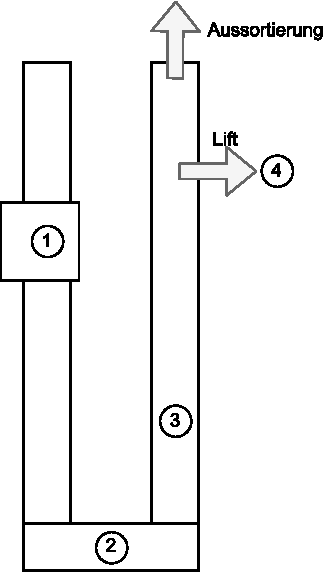
\includegraphics[keepaspectratio]{Position_Geraet}
	\caption{Mögliche Positionen des Geräts am Förderband}
\end{figure}

\subsection{Rüstplatz}
Da der Behälter während dem Entnehmen und Abfüllen des Behälters vergleichsweise lang stillsteht, hätte man an dieser Stelle sicher genug Zeit alle RFID Tags auszulesen. Mögliche Nachteile sind Platzmangel und Interferenzen durch Exemplare welche nicht im Behälter sind aber fälschlicherweise auch erfasst werden, da sie in der Nähe liegen.
\begin{itemize}
	\pro Genügend Zeit für das Auslesen aller Tags
	\pro Früh im Prozess für eine Meldung
	\con Interferenzen durch RFID markierte Exemplare in der Nähe
	\item Eventuell kein Platz für Antennen
	\item Eventuell Abschirmung/Justierung der Antennen möglich, sodass nur Exemplare im Behälter ausgelesen werden
\end{itemize}

\subsection{In einer Eckpartie}
Der Behälter führt auf dem Band zwei Rechtsdrehungen für einen Gesamtwinkel von \SI{180}{\degree} durch. An diesem Punkt bleibt der Behälter verhältnismässig lange in einem Bereich welcher von der Antenne abgedeckt werden sollte. Weiter befinden sich an dieser Position keine andere Exemplare oder Messstationen in der Nähe, was Interferenz verunmöglichen sollte.
\begin{itemize}
	\pro \textasciitilde\ drei Sekunden für das Auslesen der Tags zur Verfügung
	\pro Keine Interferenzen zu erwarten
	\con Nur beschränktes Zeitfenster
	\con Behälter in Bewegung
\end{itemize}

\subsection{Waage}
Der Behälter wird zur Bestimmung von Übergewicht gewogen, an dieser Stelle bleibt dieser etwa eine Sekunde an Ort und Stelle.
\begin{itemize}
	\pro Behälter bleibt an Ort und Stelle
	\pro Keine Interferenzen zu erwarten
	\con Nur beschränktes Zeitfenster
	\con Antenne kann nicht beliebig montiert werden
\end{itemize}

\subsection{Lift}
Der Behälter fährt vor Übergabe in das Hochregallager in einem Lift vertikal nach unten. Während dieser Zeit bleibt er längere Zeit still.
\begin{itemize}
	\pro Behälter bleibt an Ort und Stelle
	\pro Grosses Zeitfenster
	\con Beschränkter Platz da Lift
	\con Spät im Prozess
	\item Eventuell Interferenzen durch Liftmotoren
	\item Aussortierung eventuell nicht möglich
\end{itemize}

\section{Identifikation der RFID Tags}

\subsection{Eine Antenne}
\begin{itemize}
	\pro Keine Interferenzen
	\con Ausrichtung der Chips relevant
\end{itemize}

\subsection{Mehrere Antennen}
\begin{itemize}
	\pro Ausrichtung der Chips kann entgegengewirkt werden
	\pro Grössere Abdeckung
	\con Gegenseitige Interferenz
	\con Teurere Geräte nötig
	\con Mehr Platz wird benötigt
\end{itemize}

\begin{figure}
	\centering
	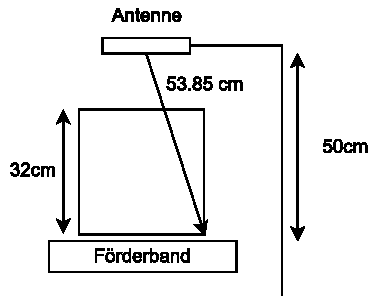
\includegraphics[keepaspectratio]{Position_Antenne}
	\caption{Positionierung einer Antenne über Förderband}
\end{figure}

\section{Identifikation des Behälters}

\subsection{Barcodeleser}
An jedem Behälter ist ein Barcode aufgeklebt (auf beiden Seiten jeweils an der richtigen Stelle, sodass die Position durch eine Drehung überführt werden kann). Durch Auslesen dieses Strichcodes ist eine Eindeutige Identifikation des Behälters möglich.
\begin{itemize}
	\pro Behälter eindeutig Identifiziert
	\pro Keine Abhängigkeiten
	\con Position muss stimmen, dass Barcode gelesen werden kann
\end{itemize}

\subsection{Bestimmung über die Mehrheit der Tags}
Falls man mehrere Tags identifiziert hat und weiss zu welchen Behältern diese gehören, kann man den nicht zum gleichen Behälter gehörenden Tag identifizieren.
\begin{itemize}
	\pro Positionsunabhängig
	\con Aktuelle Informationen über Tag und Behälter nötig (Schnittstelle Datenbank)
	\con Mindestens drei Tags müssen identifiziert worden sein
\end{itemize}

\section{Massnahmen nach Erkennungsprozess}

\subsection{Aussortierung des Behälters}
Es wäre vorstellbar, dass man den Behälter, nach einer Identifikation des Inhalts und Erkennen eines falschen Exemplars, aussortiert.
\begin{itemize}
	\pro Früh im Prozess
	\pro Wenig menschliche Interaktion für Aussortierung nötig
	\con Schnittstelle zum Steuerungssystem des Förderbands nötig
\end{itemize}

\subsection{Audiovisuelles Signal}
Man könnte eine Warnung abspielen sobald ein fehlplatziertes Exemplar identifiziert worden ist (Sirene, Warnlampe).
\begin{itemize}
	\pro Früh im Prozess
	\pro Keine Abhängigkeiten
	\con menschliche Interaktion für Aussortierung nötig
\end{itemize}

\subsection{Berichterstattung}
Man könnte, sobald ein fehlplatziertes Exemplar erkannt wurde, ein Bericht an die zuständige Stelle schicken.
\begin{itemize}
	\pro Verfolgbarkeit
	\pro Keine Abhängigkeiten zu Steuersystem
	\con Behälter muss manuell wieder aus dem Lager geholt werden
	\con Schnittstelle zu Meldesoftware nötig
\end{itemize}

\newpage

\section{Morphologischer Kasten und Variantenbeschreibung}

\begin{figure}[h!]
	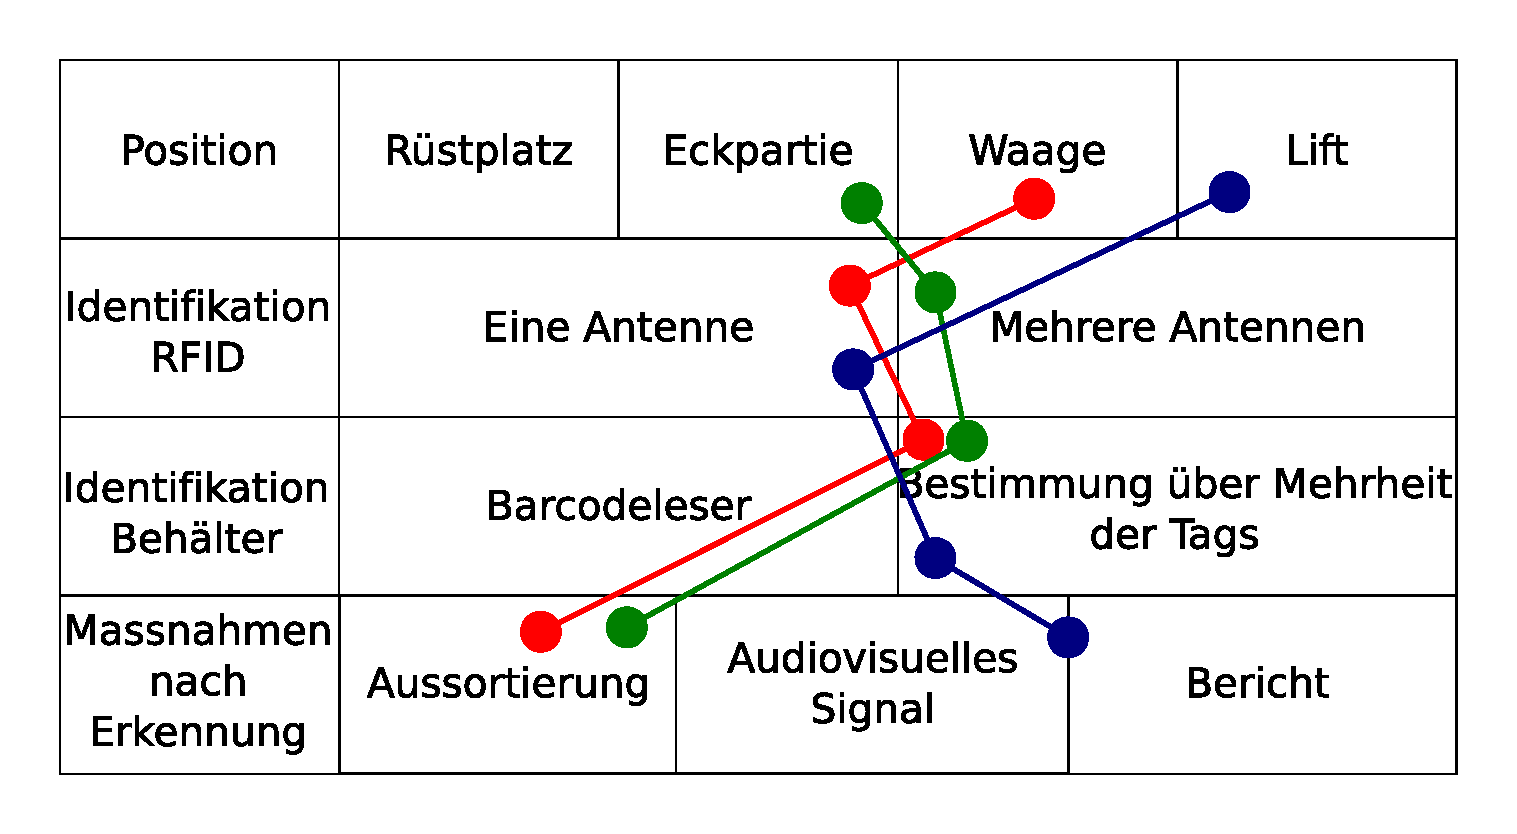
\includegraphics[keepaspectratio,width=\linewidth]{Morphologischer_Kasten}
	\caption{Die Varianten als Pfade dargestellt}
	\label{fig:MorphKasten}
\end{figure}

\subsection{Variante 1: Früherkennung und Aussortierung (Rot)}
In dieser Variante wurde Wert darauf gelegt, möglichst wenig Interferenzen zu haben, daher wurde sich für eine Antenne entschieden. Es soll über die Mehrheit der Tags der aktuelle Behälter bestimmt werden und falls Tags eines anderen Behälters gefunden wurde, der Behälter nicht eingelagert, sondern aussortiert werden (sprich ein Steuerungssignal an das Förderband gegeben werden). Der Ort wurde ausgewählt, da der Behälter dort eine kurze Pause einlegt. Diese Variante hängt stark davon ab wie schnell und fehlerfrei Tags ausgelesen werden können und ob eine Schnittstelle zur Steuersoftware existiert die wir nutzen können.

\subsection{Variante 2: Weitflächige Erkennung und Aussortierung (Grün)}
Es soll durch mehrere Antennen eine grössere Abdeckung erreicht werden und so sichergestellt werden, dass alle Tags ausgelesen werden können. Auch bei dieser Variante soll der Behälter über die Mehrheit der Tags ausgelesen werden, und dieser, wenn nötig, aussortiert werden.

\subsection{Variante 3: Erkennung und Signalisierung (Blau)}
Bei dieser Variante soll der Leser bei der Warteposition vor der Einlagerung positioniert werden, da dort die Behälter ein paar Sekunden verbleiben. Danach sollen die erkannten Tags und der Behälter als Mitteilung an die Arbeitsstation geschickt werden (Mail, Middleware, Signallampe). Das mögliche Problem dieser Variante ist, dass zwei Behälter nebeneinander in der Warteposition sein können, und dadurch allenfalls Falschpositive generiert werden können.

\section{Wahl der Variante}

Das Projektteam empfiehlt die Variante Eins, da bei dieser von wenig Interferenz ausgegangen werden kann, weil sich nur ein Behälter im Lesebereich der Antenne befindet. Weiter besteht an dieser Position auch die Möglichkeit den Behälter noch auszusortieren. Vor allem aus diesen Gründen bevorzugen wir die erste Variante.

\subsection{Übersicht der Hardwarekomponenten}

\chapter{Finanzierungsplan}

Als Berechnungsgrundlage wird ein Konzept mit einer Antenne und einer Steuerung über das Netzwerk gerechnet. Die Daten von Feig wurden von Euro auf CHF umgerechnet (Wechselkurs 1.14). Zudem sind dies die Demopreise für einen Prototyp.

\vspace{1em}

\begin{tabularx}{\textwidth}{|r|X|r|r|}
	\hline 
	\textbf{Menge} & \textbf{Produkt} & \textbf{Kosten(CHF)} & \textbf{Kosten gesamt(CHF)} \\
	\hline 
	1 & RFID Reader ID ISC.LR2500-A (Feig) & 1'200 & 1'200 \\ 
	\hline 
	1 & RFID Antennen ID ISC.ANT800/600 (Feig)& 760 & 760 \\
	\hline
	1 & RFID Antennenkabel ID ISC.ANT.C-A (Feig) & 20 & 20 \\
	\hline
	1 & Netzteil ID NET.24V-B (Feig) & 30 & 30 \\
	\hline
	1 & Netzkabel ID CAB.NET.24V-B-EU (Feig) & 4 & 4 \\
	\hline
	1 & Raspberry Pi 3 Model B+ (pi-shop.ch)& 39 & 39 \\
	\hline
	1 & Sandisk Extreme 128GB Class 10 (digitec.ch)& 45 & 45 \\
	\hline
	& & & \textbf{2098} \\
	\hline
\end{tabularx} 
